%% PNAStmpl.tex
%% Template file to use for PNAS articles prepared in LaTeX
%% Version: Apr 14, 2008


%%%%%%%%%%%%%%%%%%%%%%%%%%%%%%
%% BASIC CLASS FILE 
%% PNAStwo for two column articles is called by default.
%% Uncomment PNASone for single column articles. One column class
%% and style files are available upon request from pnas@nas.edu.
%% (uncomment means get rid of the '%' in front of the command)

%\documentclass{pnasone}
\documentclass{pnastwo}

%%%%%%%%%%%%%%%%%%%%%%%%%%%%%%
%% Changing position of text on physical page:
%% Since not all printers position
%% the printed page in the same place on the physical page,
%% you can change the position yourself here, if you need to:

% \advance\voffset -.5in % Minus dimension will raise the printed page on the 
                         %  physical page; positive dimension will lower it.

%% You may set the dimension to the size that you need.

%%%%%%%%%%%%%%%%%%%%%%%%%%%%%%
%% OPTIONAL GRAPHICS STYLE FILE

%% Requires graphics style file (graphicx.sty), used for inserting
%% .eps files into LaTeX articles.
%% Note that inclusion of .eps files is for your reference only;
%% when submitting to PNAS please submit figures separately.

%% Type into the square brackets the name of the driver program 
%% that you are using. If you don't know, try dvips, which is the
%% most common PC driver, or textures for the Mac. These are the options:

% [dvips], [xdvi], [dvipdf], [dvipdfm], [dvipdfmx], [pdftex], [dvipsone],
% [dviwindo], [emtex], [dviwin], [pctexps], [pctexwin], [pctexhp], [pctex32],
% [truetex], [tcidvi], [vtex], [oztex], [textures], [xetex]

\usepackage{graphicx}
\usepackage[space]{grffile}
\usepackage{latexsym}
\usepackage{amsfonts,amsmath,amssymb}
\usepackage{url}
\usepackage[utf8]{inputenc}
%\usepackage{hyperref}
%\hypersetup{colorlinks=false,pdfborder={0 0 0}}
\usepackage{textcomp}
\usepackage{longtable}
\usepackage{multirow,booktabs}
%\usepackage{multicol}
%%%%%%%%%%%%%%%%%%%%%%%%%%%%%%
%% OPTIONAL POSTSCRIPT FONT FILES

%% PostScript font files: You may need to edit the PNASoneF.sty
%% or PNAStwoF.sty file to make the font names match those on your system. 
%% Alternatively, you can leave the font style file commands commented out
%% and typeset your article using the default Computer Modern 
%% fonts (recommended). If accepted, your article will be typeset
%% at PNAS using PostScript fonts.


% Choose PNASoneF for one column; PNAStwoF for two column:
%\usepackage{PNASoneF}
%\usepackage{PNAStwoF}

%%%%%%%%%%%%%%%%%%%%%%%%%%%%%%
%% ADDITIONAL OPTIONAL STYLE FILES

%% The AMS math files are commonly used to gain access to useful features
%% like extended math fonts and math commands.

%%%%%%%%%%%%%%%%%%%%%%%%%%%%%%
%% OPTIONAL MACRO FILES
%% Insert self-defined macros here.
%% \newcommand definitions are recommended; \def definitions are supported

%\newcommand{\mfrac}[2]{\frac{\displaystyle #1}{\displaystyle #2}}
%\def\s{\sigma}

\def\i{^{(i)}}
\def\xopt{\vx_\star}
\def\xrec{\widetilde\vx}
\def\X{\calX}
\def\D{\calD}
\def\H{\mathrm{H}}
\newcommand{\x}{\mathbf{x}}
\newcommand{\EI}{\textrm{EI}}
\newcommand{\C}{\mathcal{C}}
\newcommand{\given}{\,|\,}
\newcommand{\DistGam}{\text{Gam}}


  

%%%%%%%%%%%%%%%%%%%%%%%%%%%%%%
%% Don't type in anything in the following section:
%%%%%%%%%%%%
%% For PNAS Only:
\contributor{Submitted to Proceedings
of the National Academy of Sciences of the United States of America
\url{www.pnas.org/cgi/doi/10.1073/pnas.0709640104}}
\copyrightyear{2008}
\issuedate{Issue Date}
\volume{Volume}
\issuenumber{Issue Number}
%%%%%%%%%%%%

% Close the \begin{article} auto-opened by Authorea, if the author hasn't done so already
\usepackage{etoolbox}
\newbool{InArticleEnvironment}
\AtBeginEnvironment{article}{\booltrue{InArticleEnvironment}}
\AtEndDocument{\ifbool{InArticleEnvironment}{\end{article}}{}}

\begin{document}

\title{Large-scale Accelerated Exploration of Chemical Space with Bayesian Neural Networks}

\author{Jos\'e Miguel Hern\'andez-Lobato\affil{1}{Harvard University}, Edward O. Pyzer-Knapp\affil{1}{Harvard University}, 
Ryan P. Adams\affil{1}{Harvard University} \and Al{\'a}n Aspuru-Guzik\affil{1}{Harvard University}}

\contributor{Submitted to Proceedings of the National Academy of Sciences
of the United States of America}

\maketitle

\begin{article}

\begin{abstract} 
Chemical space is so large as to make brute force searching for molecules with
improved properties infeasible. Adaptive design can accelerate the discovery
process by sequentially identifying the most useful experiments to be performed
next. However, existing adaptive design methods have shortcomings that limit
their applicability to the molecule search problem. First, they lack
scalability and cannot work with the large amounts of data that are required to
successfully navigate chemical space. Second, they are unable to learn feature
representations for the data, which reduces their statistical efficiency. To
avoid these limitations, we propose an alternative approach based on the
combination of Bayesian neural networks with probabilistic active learning. Our
methods are computationally and statistically efficient by leveraging on recent
advances in approximate Bayesian inference. Maximum entropy sampling is used
to find small sets of molecules with good extrapolation properties. Thompson
sampling is used to quickly identify molecules with improved properties. Our
techniques generate enriched libraries of compounds in a fraction
of the time required by a stochastic (Monte Carlo) search approach and with
more robustness than a purely greedy search strategy.
\end{abstract}

%\keywords{monolayer | structure | x-ray reflectivity | molecular electronics}

%\abbreviations{SAM, self-assembled monolayer; OTS, octadecyltrichlorosilane}

\bibliographystyle{pnas}

\section{Introduction}

Chemical space is huge, with estimates of over $10^{60}$ molecules. Among
these, less than 100 million compounds are found in public repositories or
databases \cite{reymond_enumeration_2012}. This means that many molecules with
useful function for man-kind are still to be discovered (e.g., new energy
materials, pharmaceuticals, dyes, etc.). The vast size of chemical space makes,
however, very challenging to search for new relevant compounds among the many
unimportant ones. Because of this, a discovery process relaying only on
the combination of scientific intution with trial and error experimentation is slow and tedious.

To accelerate the search, high-throughput approaches can be used in a
combinatorial exploration of small specific areas of chemical space
\cite{rajan_combinatorial_2008}. These have led to the development of
high-throughput virtual screening
\cite{pyzer-knapp_what_2015,halls_highthroughput_2010,
curtarolo_highthroughput_2013,husch_largescale_2015,subramaniam_virtual_2008,shoichet_virtual_2004,
jain_commentary_2013}, in which large libraries of molecules are analyzed using
theoretical and computational techniques and then reduced to a small set of
promising leads that experimentalist can follow up on. With masive initial libraries, these methods are already
hitting the limits of modern computation---even though they search only a small
drop in the ocean of chemical space. Therefore, at present, there is an urgent
need to accelerate high-throughput screening approaches.

Machine learning (ML) tools can be used for such purpose. These methods can
extrapolate the fitness values of a reduced set of molecules for which data has
already been collected to a much larger set of molecules.  ML techniques can
produce a significant acceleration of the screening process because their
predictions are much faster to compute than the calculations required to
evaluate each molecule's fitness.

Neural networks are ML methods that have been considered by the chemistry
community for solving the aforementioned data prediction problem
\cite{zupan_neural_1991, burden_using_1996,
rodemerck_application_2004,myint_molecular_2012,DuvMacetal15nfp}. As an example, neural networks  were used
recently to predict the efficiency of a large set of organic
photovoltaics generated by combinatorial methods
\cite{pyzer-knapp_learning_2015-1}. In this work, the neural network
predictions were used to discard 99\% of the molecules in the initial
library, saving many expensive computations.

Although the above results are promising, higher speed-ups can in principle be
obtained with adaptive design tools \cite{jones1998efficient}. These techniques
use ML predictions to guide the search and make optimal decisions about what
molecules to analyze next given the data collected so far. The key idea is to
attain a balance between exploration and explotation in the molecule selection
process. On one hand, we would like to analyze next molecules with high
expected fitness as estimated by the ML method (exploitation). On the other
hand, we would also like to select next molecules for which the ML predicctions
are uncertain, since collecting such data is likely to improve the quality of
the predictions in the long run (exploration). For efficient
exploration, it is important to use ML methods that produce accurate
estimates of uncertainty in their predictions. 
Adaptive design tools achieve a balance
between the objectives explotation and exploration in an iterative loop with
feedback from experiments. 
The result is a general, principled and robust
approach for accelerating the discovery process. 
Figure ? shows the iterative
feedback loop used by adaptive design techniques.

Several studies have already applied adaptive design tools to the search for
molecules with improved properties
\cite{xue2016accelerated,negoescu2011knowledge,de2008active}. However, these
works are hampered by several limitations. First, the proposed methods are only
applied in the small-data regime, with measurements collected for at most one
thousand molecules---while current high-throughput studies can collect data for
millions of molecules. The reason for using small amounts of data is that these
adaptive design methods relay on the predictions generated by Gaussian
processes (GPs) \cite{rasmussen2006gaussian}, which are ML techniques that
produce accurate estimates of uncertainty but also have a high computational
cost. GPs can be scaled up by using approximations based on inducing inputs
\cite{snelson2005sparse,hensman2015scalable}. However, these methods become
statistically inefficient in the large-data regime because they cannot learn
feature representations for the data \cite{bengio2007scaling}.
Neural networks do not have these disadvantages. They are highly scalable and
by using adaptive basis functions, they can make very accurate predictions with
large amounts of data \cite{lecun2015deep}. However, it is in general very
difficult to produce

also have very good predictive performance
with large amounts of data because they can

the accuracy predictions tend to


 and tend to produce


models 

approximations

complexity, but are

which 

 methods


and only collect measurement for less than a few thousand molecules.
The reason for this is that they

use use kernel methods


are limited by considering only ML methods that 
do not scale to large amounts of data and that 
that are required to
successfully navigate chemical space. Second, they are unable to learn feature
representations for the data, which reduces their statistical efficiency. 

have been used so far


 on average,

, but also 

give high fitness values

select molecules according to a balance 

molecules for which the ML
predictions 

predict best

ing 

the merits of searching for materials likely to
have the best property or where there may be fewer sampling
points and greater uncertainty, but which may improve the
quality of the regressor in the long run.

Hence, an approach is needed, which can adaptively guide the next experiments. 

That is, an
adaptive procedure that makes optimal choices of materials to test
next by balancing the merits of searching for materials likely to
have the best property or where there may be fewer sampling
points and greater uncertainty, but which may improve the
quality of the regressor in the long run. Adaptive design has been
successfully  applied  in  areas  spanning  computer  science



without requiring expensive simulations --- aside from those used for
generating the training set. 

Up until this point, the sets of molecules used for training these models have been generated via random exploration; which is known to be inefficient.  In this study we show how the use of active learning techniques can allow the generation of highly predictive neural networks on a fraction of the data previously used. We will also demonstrate how Thompson sampling\cite{thompson_likelihood_1933} can be used to perform an `intelligent search' of chemical libraries, picking out high-potential molecules efficiently; thus significantly increasing the scope for high-throughput virtual screening and moving towards the ultimate goal of optimization in chemical space.

We will begin by describing Bayesian neural networks, and the active learning techniques we have used for intelligently searching chemical  space.  We will then describe the three libraries which we have used to demonstrate the advantages of using intelligent searching techniques through an analysis of the diversity measured using a neural network.  We will then  discuss the results of both active learning techniques when applied to these data sets, illustrating the power of searching in an intelligent manner. 

\section{Methods}

Any intelligent method of exploring chemical space must balance exploration of a wide range of molecules (often thought of in terms of diversity maximization\cite{Blaney_1997,Wang_2009,Fitzgerald_2006,reker_activelearning_2015}) with exploiting the predictive power of the method used. We note that random searches have been used for the exploration of chemical spaces\cite{23548177}, and include results for a random search as a benchmark for these methods, since for a method to approach `intelligence', it surely must give significant improvements in efficiency over a random (Monte Carlo) regime.

\subsection{Bayesian Neural Networks}

When implementing an intelligent search, it is desirable to utilize a predictive method as a fast approximation to either an expensive calculation, or an experimentally observed value.  Additionally, since the goal is the large scale exploration of chemical space, the method must also possess good scaling characteristics.  In this regard, neural networks provide an ideal solution.  Neural networks are known to produce state-of-the-art results for predicting chemical properties \cite{ma2015deep,unterthiner2015toxicity,ramsundar2015massively}, and they can also be applied to large datasets by using stochastic optimization techniques \cite{bousquet2008tradeoffs}. 

In order to balance exploration and exploitation, it is desirable to utilize a probablistic prediction paradigm, rather than the more common deterministic prediction.  Making probabilistic predictions with neural networks is traditionally a difficult task; we make use of a recent breakthrough in the scalable training of Bayesian neural networks developed by some of the authors \cite{hernandez2015probabilistic}, known as probablistic back propagation (PBP). 

In a neural network with~$L$ layers, where~$V_l$ is the number of hidden units in layer~$l$, and~${\mathcal{W} = \{ \mathbf{W}_l \}_{l=1}^L}$ is the collection of~${V_l\times (V_{l-1}+1)}$ weight matrices between fully-connected layers. The $+1$ is introduced to account for the additional per-layer biases. We denote the outputs of the layers by vectors~$\{ \mathbf{z}_l \}_{l=0}^{L}$, where~$\mathbf{z}_0$ is the input layer,~${\{\mathbf{z}_l\}_{l=1}^{L-1}}$ are the hidden units and~$\mathbf{z}_L$ denotes the output layer, which is one-dimensional since the target variables $y_n$ are scalars.  
The input to the $l$-th layer is defined as~${\mathbf{a}_l = \mathbf{W}_l \mathbf{z}_{l-1} / \sqrt{V_{l-1}+1} }$,
where the factor~${1/\sqrt{V_{l-1} + 1}}$ keeps the scale of the input to each neuron independent
of the number of incoming connections.
The activation functions for each hidden layer are rectified linear units (ReLUs)
\cite{nair2010rectified}, i.e.,~${a(x) = \max(x,0)}$.
Let $\gamma$ be the precision of the Gaussian noise in the target variables and let $\lambda$
be the precision of the zero-mean isotropic Gaussian prior on the network weights.
PBP approximates the posterior distribution on $\mathcal{W}$, $\gamma$ and $\lambda$ with
the tractable distribution
\begin{multline}
q(\mathcal{W},\gamma, \lambda) = \textstyle \left[ \prod_{l=1}^L\! \prod_{i=1}^{V_l}\! 
\prod_{j=1}^{V_{l\!-\!1}\!+\!1} \mathcal{N}(w_{ij,l}| m_{ij,l},v_{ij,l})\right ]
\\ \DistGam(\gamma\given \alpha^\gamma, \beta^\gamma)
\DistGam(\lambda\given \alpha^\lambda, \beta^\lambda)\,.\label{eq:posterior_approximation}
\end{multline}
PBP tunes the parameters of $q$ by iterating an assumed
density filtering (ADF) algorithm over the training data \cite{opper1998bayesian}. The main operation in PBP
is the update of the mean and variance parameters of (\ref{eq:posterior_approximation})
each time a new data point is processed. 

\begin{figure}[hb]
\centering
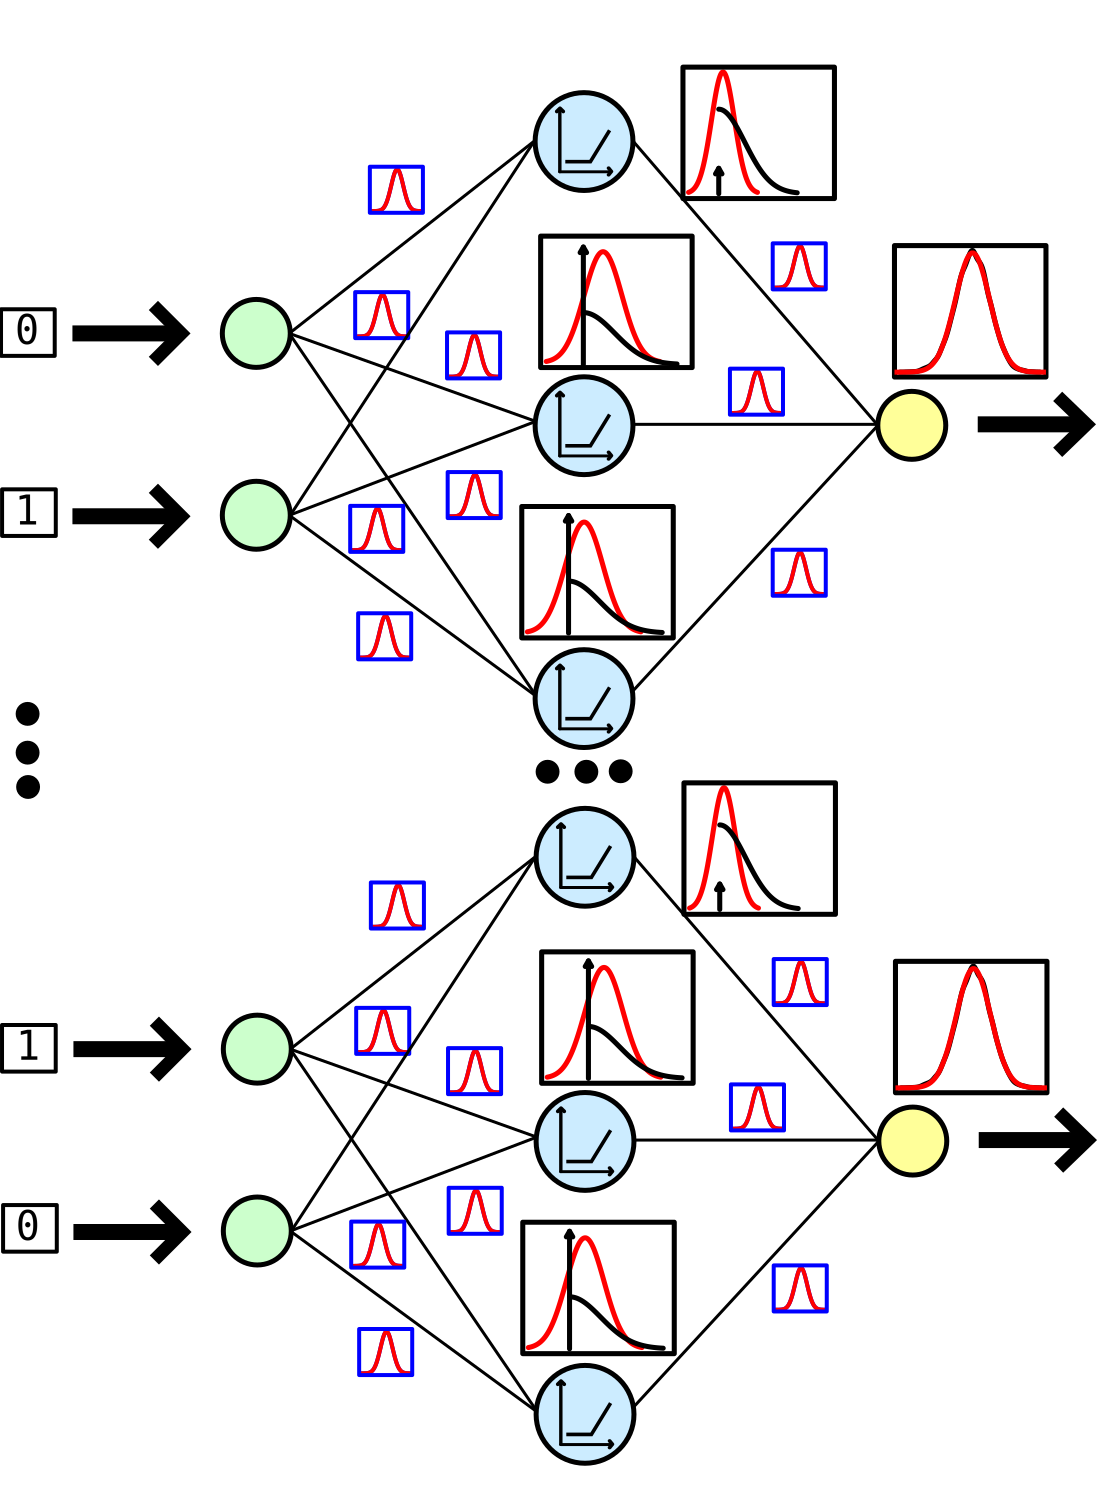
\includegraphics[width=0.8\columnwidth]{figures/pbp.png}

\caption{A graphical representation of the probabalistic back propagation (PBP) algorithm. Deterministic inputs, here represented as $1$s and $0$s are passed through the Bayesian neural network. The main operation in PBP is the update of the mean and variance parameters of the posterior approximation each time a new data point is processed. Updates are propagated using moment matching between the old and new liklihoods, with ADF Gaussian updates.}
\label{fig:pbp}
\end{figure} 
For this, PBP matches moments between
the new $q$ and the product of the old $q$ and the likelihood factor
$\mathcal{N}(y_n\given f(\mathbf{x}_n;\mathcal{W}),\gamma^{-1})$,
where $f(\mathbf{x}_n;\mathcal{W})$ denotes the output of the network for input $\mathbf{x}_n$ and weight values $\mathcal{W}$.
The matching of moments for the weights is achieved by using standard ADF Gaussian updates (see
\cite{minka2001family}, equations 5.12 and 5.1):
\begin{align}
m_{ij,l}^\text{new} & = m_{ij,l} + v_{ij,l} \nabla_{m_{ij,l}} \log Z \,,\label{eq:adf_update_1}\\
v_{ij,l}^\text{new} & = v_{ij,l} - v_{ij,l}^2 \left[ (\nabla_{m_{ij,l}} \log Z)^2 - 2 \nabla_{v_{ij,l}} \log Z \right]\,,\label{eq:adf_update_2}
\end{align}
where $Z$ is the result of marginalizing the likelihood $\mathcal{N}(y_n\given f(\mathbf{x}_n;\mathcal{W}),\gamma^{-1})$ with
respect to $q$. The computation of $Z$ is intractable. However, PBP circumvents this problem by
approximating the distribution of the network output $f(\mathbf{x}_n;\mathcal{W})$ when $\mathcal{W} \sim q$ with a Gaussian. 
This is achieved in a forward pass through the network where each non-Gaussian distribuion
for the output of each neural unit is approximated with a Gaussian by moment matching.
When $\gamma\sim q$, the marginalization of $\mathcal{N}(y_n\given f(\mathbf{x}_n;\mathcal{W}),\gamma^{-1})$ 
with respect to $\gamma$ produces a Student's $t$ density which does not
convolve in closed form with respect to the Gaussian approximation on $f(\mathbf{x}_n;\mathcal{W})$. Neverheless, this Student's
$t$ density can be as well approximated with a Gaussian by moment matching to obtain a closed form convolution that approximates $Z$.
The gradients required in (\ref{eq:adf_update_1}) and (\ref{eq:adf_update_2}) can then be obtained by backpropagation.
After several ADF iterations over the data,  we can obtain a probabilistic
prediction for $f(\mathbf{x}_\star;\mathcal{W})$ given the test input
$\mathbf{x}_\star$ by applying the forward pass process described above.  We
refer the reader to \cite{hernandez2015probabilistic} for full details on PBP; a graphical depiction of the process of training a Bayesian neural network using PBP is shown in Figure \ref{fig:pbp}.


\subsection{Active learning}

When navigating chemical space, there are two main tasks of interest.  The first one is to find a model with low prediction error as quickly as possible.
This is particularly helpful when we need accurate predictions over a wide range of possible inputs. One potential case in which that is important is the prediction of toxcity.  Here, the accuracy of a model is important and  also not a classic optimization problem. For this first task we propose to use the maximum entropy sampling heuristic, which can be shown to select the most informative molecules for solving
the prediction problem.  The second task is a classic optimization challenge --- we want to find molecules that achieve high values for some fitness
function.  In some cases this may be one molecule, but in many --- especially in high-throughput screening scenarios \cite{pyzer-knapp_what_2015} --- the
desired outcome is to find the most enriched set of molecules. For this task, we propose to use Thompson sampling \cite{thompson_likelihood_1933}, a simple
heuristic that achieves a strong balance of exploration and exploitation \cite{Chapelle2011}.

\subsubsection{Maximum entropy sampling}

In the paradigm of probabalistic sampling, the best way to quickly reduce the error in a model is to collect maximally informative molecules. To actively collect the most informative molecules we follow an information-based approach \cite{Mackay1992}. The goal is to maximize the expected reduction in posterior entropy that is produced by adding data to the training set. This implies choosing the data point~$\mathbf{x}$ that maximizes
\begin{align}
\text{H}[\mathbf{w}|\mathcal{D}] - 
\mathbb{E}_{y|\mathbf{x},\mathcal{D}}\text{H}[\mathbf{w}|\mathcal{D}\cup\{\mathbf{x},y\}]\,,\label{eq:acquisition_function}
\end{align}
where~$\text{H}[\cdot]$ is the differential entropy,~$\mathbf{w}$ are the model parameters,~$\mathcal{D}$ is the data collected so far and~$y$ is the unknown target associated with~$\mathbf{x}$. We can rewrite~(\ref{eq:acquisition_function}) by swapping the roles of~$y$ and~$\mathbf{w}$~\cite{houlsby2012collaborative}:
\begin{align}
\text{H}[y | \mathbf{x},\mathcal{D}] - 
\mathbb{E}_{\mathbf{W} | \mathcal{D}}\text{H}[y | \mathbf{w}\mathbf{x}]\,.\label{eq:new_acquisition_function}
\end{align}
Since the last term in~(\ref{eq:new_acquisition_function}) is constant, we select the~$\mathbf{x}$ that maximizes the entropy of the predictive distribution~$p(y| \mathbf{x},\mathcal{D})$. When $p(y| \mathbf{x},\mathcal{D})$ is Gaussian, we select the~$\mathbf{x}$ with highest predictive variance.

\subsubsection{Thompson sampling}

Thompson sampling (TS) \cite{thompson_likelihood_1933} is a simple heuristic for efficiently identifying the optimal element in a set. Solving this problem
requires to find an optimal exploration/explotation trade-off. A strong property of TS  is that this is performed automatically without the need for the introduction of additional parameters, which would themselves require optimization. 
We achieve this with the following algorithm:
\begin{enumerate}
\item A very small number of molecules are selected randomly, and ground truth values are calculated
\item A Bayesian neural network is trained with PBP on this training data
\item The model parameters are sampled from their posterior distribution, providing a set of deterministic neural networks
\item Each deterministic neural network makes predictions for all the remaining molecules. 
\item For each deterministic neural network, the set of unique molecules with highest score is selected,  ground truth values calculated, and added to the training set.
\item Steps 2-5 are repeated
\end{enumerate}
By sampling the weight distributions in the Bayesian neural network, we produce a set of deterministic neural networks, the weights of which vary across the set in a manner directly related to the uncertainty of the probabalistic model in their value.  Thus, a balance in the search for extreme molecules is achieved without directly imposing any external measure of molecular diversity - which is in itself an area of intense study\cite{Maldonado_2006}.
  
  

\section{Desciptions of the Data Sets}
The input features for all molecules in the data set were 512-bit Morgan circular fingerprints\cite{Rogers_2010}, calculated with a bond radius of 2, and derived from the canonical smiles, implemented in the RDkit\cite{rdkit}.

\textbf{Harvard Clean Energy Project}:The Clean Energy Project is the world's largest materials high-throughput virtual screening effort\cite{hachmann_lead_2014,hachmann_harvard_2011}, and has scanned more than 3.5 million molecules to find those with high power conversion efficiency (PCE) using quantum-chemical techniques, taking over 30,000 years of CPU time. The target value within this dataset is the power conversion efficiency (PCE), which is calculated for the 2.3 million publicly released molecules, using the Scharber model\cite{scharber_design_2006} and frontier orbitals calculated at the BP86\cite{perdew_density-functional_1986,becke_densityfunctional_1993}\/def2-SVP\cite{weigend_balanced_2005} level of theory.


\textbf{Dose-Response Data Set}:These data sets were obtained from the NCI-cancer database\cite{_nci_}.  The dose-response target value has a potential range of -100 to 100, and reports a percentage cell growth relative to a no-drug control.  Thus, a value of +40 would correspond to a 60\% growth inhibition and a value of -40 would correspond to 40\% lethality.  Molecules with a positive value for the dose-response are known as inhibitors, molecules with a score less than 0 return a cytotoxic effect. Results against the NCI-H23 cell line was taken against a constant log(concentration) of -8.00M and where multiple identical conditions were present in the data, an average was used.  It should be noted that for this data set, we assert smaller values represent a more desirable outcome. 


\textbf{Malaria Data Set}:The Malaria data set was taken from the \textit{P. falciparum} whole cell screening derived by combining the GSK TCAMS data set, the Novatis-GNF Malaria Box data set and the St Jude's Research Hospital data set, as released through the Medicines for Malaria Venture website \cite{23798988}.  The target is the EC50 value, which is defined as the concentration of the drug which gives half maximal response.  Much like the Dose response set, this is a minimization problem; the lower the concentration, the more potent the drug.

\subsection{Data Set Analysis via Dimensionality Reduction with Neural Networks - Information Landscapes}
When analyzing data sets for qualities such as diversity, it is important to make the distance measure consistent with the predictive model.  For example, if the prediction were made with a Gaussian process, it would be wise to use the distance model built into the kernel to analyze the diversity of the datasets studied.  This becomes somewhat more complex when the predictive method does not have a well defined distance measure built into it, such as a neural network.  Simply analyzing the diversity of the inputs through the use of a Tanimoto distance histogram, for example, is potentially a dangerous path since it does not acknowledge the highly connected nature of the neurons in a neural network.  We instead utilize an alternative measure, in which a neural network itself is used to compress the data into a resonable number of dimensions,~\cite{hinton_reducing_2006} upon which a visual inspection can reveal the diversity of the dataset.

This is achieved through training an unsupervised neural network, of which the loss function of each layer is determined by how well the output matches that of the previous layer.  Through sequential reduction in the number of neurons, the principle components of an input signal are amplified, and can be sampled.  To fine tune the weights of this neural network, the funneling architecture is mirrored, and the weights adjusted so that a loss function comparing the input and output of the network is minimized.  
\begin{figure}[h!]
\centering
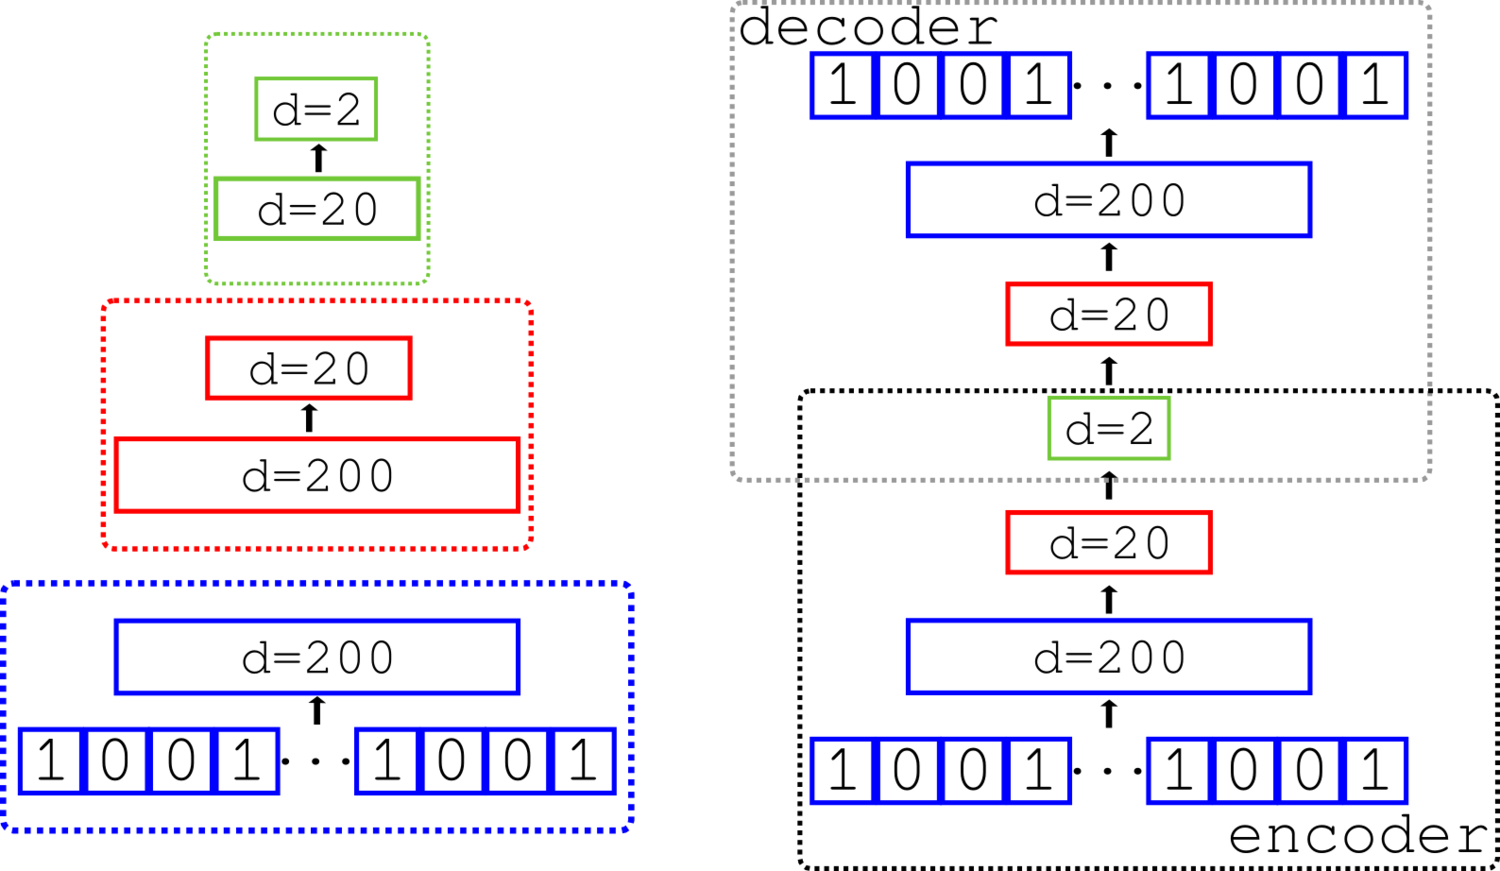
\includegraphics[width=1\columnwidth]{figures/nnet_decomp.png}
\caption{Neural networks can be used to compress data into a few, representative directions. In order to properly condition the weights of the neural network to be close to an optimal solution, the weights of each layer are pre-trained so that the layer reproduces the output of the previous layer (left).  These layers are then stacked into a funnel first decreasing in size (the encoder) and then increasing in size (the decoder).  Finally, the weights are fine-tuned to minimize reconstruction error (right).}
\label{fig:nn_decomp}
\end{figure}
The distributions of these network derived principle components were further investigated through the calculation of pairwise component distances. These distances were normalized so that the maximum distance was set at 1.0, and the minimum set to be 0.0. It can be seen from Figure \ref{fig:dist_hists}, that all of the sets are reasonably diverse in the eyes of the neural network.  As seen from figure 3, these sets are reasonably diverse in the eyes of the neural network. This statement may be counterintuitive from the chemical perspective, as perhaps one can think that molecules to carry out a specific task are likely to be more chemically similar. Global diversity measures can often give a misleading view into how models work on data. These measures can be thought of as a map of the local surroundings in chemical space.  To extend the metaphor, if you are looking to find the best place for a picnic, it is more helpful to have a streetmap than a globe.
  
  

\begin{figure}[h!]
\centering
\includegraphics[width=1\columnwidth]{figures/NN_distances_all/NN_distances_all.png}
\caption{The distribution of pairwise component distances, as calculated through the neural-network based procedure.  The distances were normalized to be in the range 0 to 1, where 1 is the maximal distance between two sets of components.  The histogram (top) was set to contain 100 bins, and is complemented below by a violin plot, in which the 25th, 50th and 75th percentiles are marked.  A violin plot is similar to a box-plot, but its width at any point is derived from a kernel density estimate of the underlying data.}
\label{fig:dist_hists}
\end{figure}

The underlying information derived from these network derived components can be further investigated through the use of a plot we call an 'information landscape'.  In this plot, chemical space (as described by the components, which are bound between 0 and 1) is split into areas of size 0.2x0.2 arbitrary units. The mean value for the targets contained within each area is calculated, and determines the color of that area.  In order to visualize the distribution of molecules within this depiction of chemical space, a kernel density estimate is used to plot contour lines.  Additionally, the top 100 molecules, ranked according to their target value, are plotted as points on the surface.  By analyzing the distribution of the data, alongside the location of extreme molecules, it is easy to classify the data into types of information landscape.  In Figure \ref{fig:info_landscapes}, we can see the information landscapes created to describe each of the data sets used within this study.  The Clean Energy Project dataset is striking in the strength of the input/property relationship --- the majority of the top molecules are concentrated in a relatively small area of chemical space.  Additionally, in this dataset, there is a clear trend for worsening performance as the Y-axis is ascended.  This is not the case for the other two datasets, in which the `good' areas of chemical space are more randomly distributed.  It is interesting to observe the One-Dose data set, in which there are two clear families of extreme molecules, one towards the top of the plot and one towards the bottom left.  This could be indicative of two different approaches taken in the literature to approach the problem of developing good treatments for this particular type of cancer. 
\begin{figure}[htb]
\centering
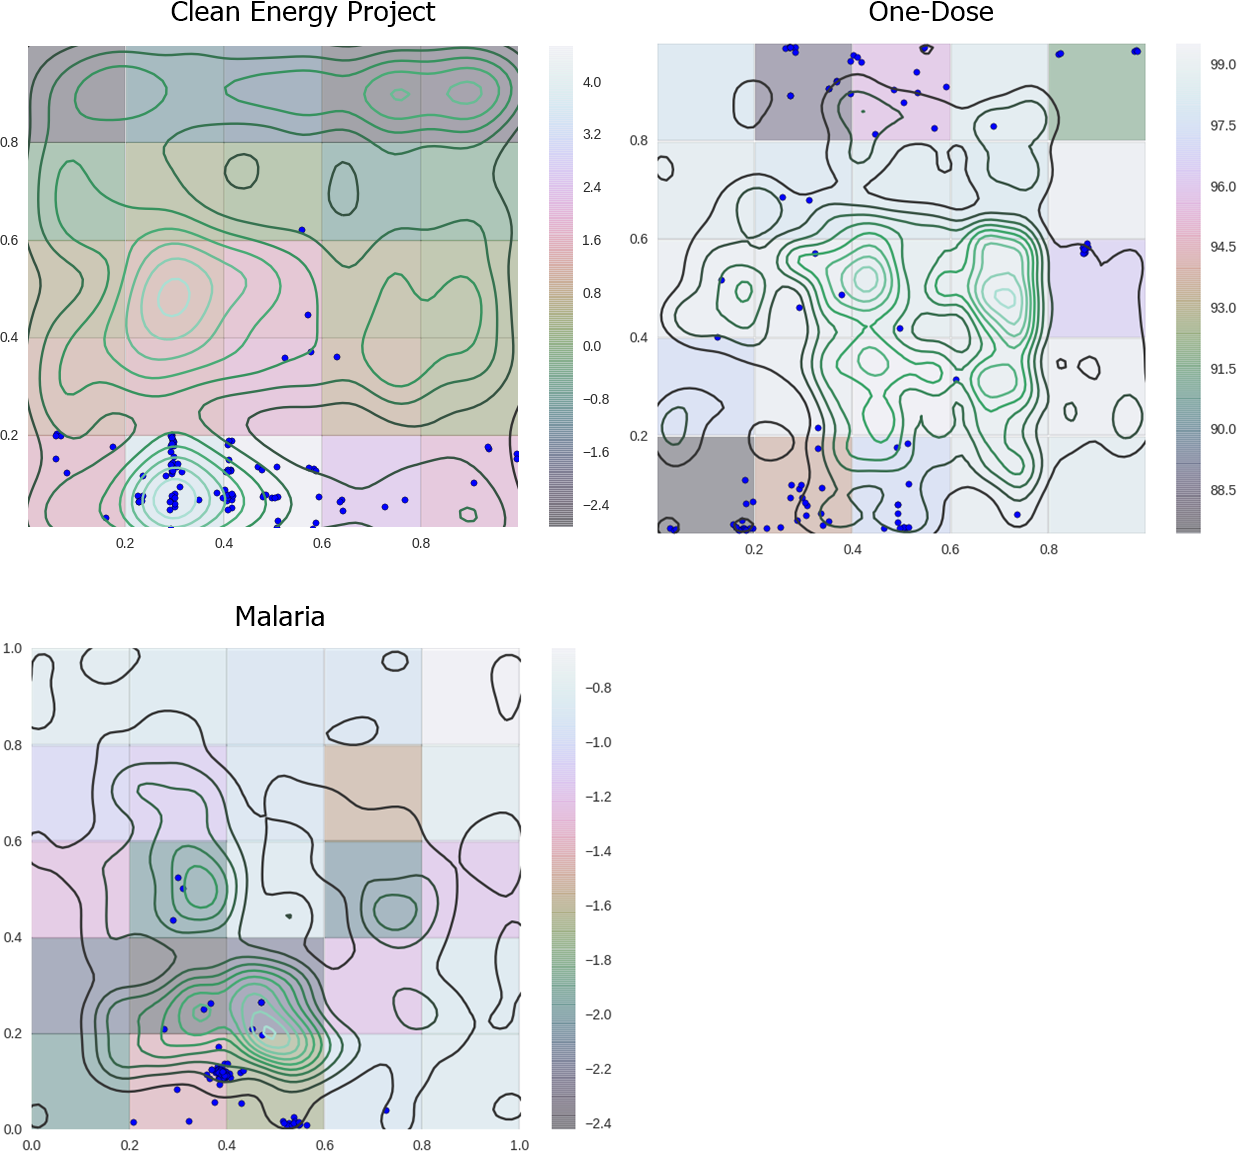
\includegraphics[width=\columnwidth]{figures/info_landscape-tile/info_landscape-tile.png}
\caption{Information landscapes for the Clean Energy Project, One-Dose and Malaria datasets.  The colors represent the mean value of targets whose reduced dimensional inputs fall within that area of reduced feature space, the contour lines are a kernel density estimate of the location of inputs, and the blue dots represent the location of the reduced dimensional features which represent the top 100 target values for each set.}
\label{fig:info_landscapes}
\end{figure}

\section{Results and Discussion}
\subsection{Maximum Entropy Sampling}

Due to the size of the datasets in this study, at each sampling stage we draw multiple molecules - 200 for the malaria and one-dose datasets which both contain around 20,000 molecules - and 1000 for the CEP dataset, which contains 2 million molecules. Additionally for the CEP dataset, in order to penalize adding sets of molecules which are very similar (and thus contribute less to the entropy) we remove redundent molecules by applying a clustering based upon the Tanimoto distance, with molecules being clustered with a tolerance of 0.9 distance and only one representative of each cluster added to the training set.  The effect of removing redundant molecules is particularly strong in very large datasets such as the CEP, and whilst we tested this method on the other data sets, we found that it had little or no effect upon the outcome, so for these datasets we report the results without the clustering.


For each of the results shown in Figure \ref{fig:max_entropy}, it can be seen that actively collecting molecules using the maximum entropy sampling methodology affords an improvement in the speed of discovery of maximally informative sets of molecules, with the RMSE curve both dropping much faster to a low error, compared to the Monte Carlo sampling.  For the largest of these sets, the CEP Data Set, the trajectory of this sampling is much noisier for the Monte Carlo sampler, than the maximum entropy sampler.  The smoothness of the maximum entropy sampler is important when considering the application of these methods in `live' situations; sampling 
\begin{figure}[ht]
\centering
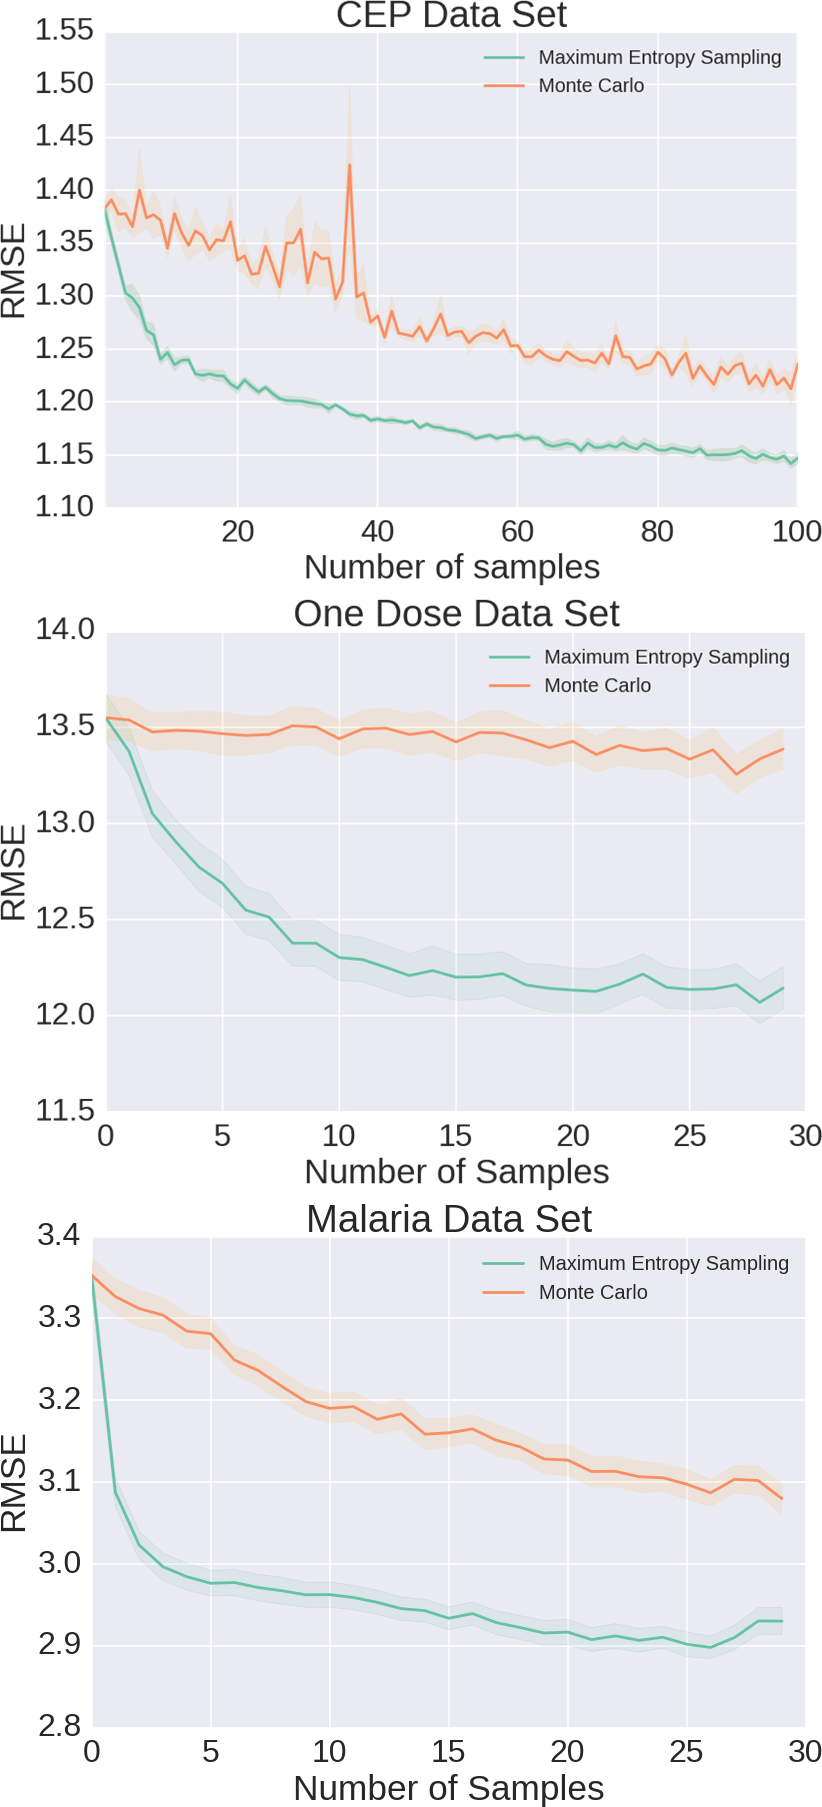
\includegraphics[width=0.8\columnwidth]{figures/mes_tile1/mes_cep-vert3.png}

\caption{The results of maximum entropy sampling for the three datasets included in this study.  It can be seen that for all three datasets, selecting the molecules actively using maximum entropy sampling results in a lower root-mean-squared-error (RMSE) at lower sample counts than randomly sampling the data (Monte Carlo). The experiment was performed 50 times, allowing the calculation of errors via the bootstrapping methodology at the 95th percentile (p=0.05).}
\label{fig:max_entropy}
\end{figure}  

This result is not surprising when the distribution of pairwise distances derived using the network based components is considered. The result is most pronounced for the Malaria dataset and the One-Dose dataset, which show the most skewed distribution.  The One-Dose dataset has the lowest mean of the three sets, which suggests that molecules picked randomly will most likely have a small 'component distance', this suggests that they will be similar in the eyes of the neural network, and thus contribute little information entropy to the training set. Whilst the Malaria dataset has a higher mean, it exhibits a long-tailed distribution, which is again problematic for a Monte Carlo sampling approach.  In comparison to those, pairwise distances within the Clean Energy Project dataset are fairly close to being normally distributed.  This is realized in the results of the sampling, where Monte Carlo - despite displaying significantly more variance in its performance - does not perform as poorly when compared to the maximum entropy sampling methodology.

It is also worthwhile recalling that this method selects molecules without considering their contribution to the overall error of the training set; instead utilizing the predictive uncertainty of the model for selecting which molecules to add to the training set. Thus, it represents a purely information-based approach and clearly demonstrates the power of exploiting the underlying information landscape for intelligently constructing informative libraries. 

\subsection{Thompson Sampling}

When there is a clear target for optimization, Thompson sampling represents a strong method for exploiting the predictive power of the model, whilst also exploring relevant areas of chemical space. In order to measure the effectiveness of Thompson sampling in an high throughput virtual screening setting, we calculate the 1\% recall - that is the fraction of the top 1\% of molecules by target value which have been selected at each sample.  We can also calculate a \textit{dynamic recall}, which is the fraction of the sampled molecules which have values in the top 1\% of those contained within the entire set. 

It can be seen from Figure \ref{fig:thompson_1pc} that the Thompson sampling methodology significantly outperforms the Monte Carlo, and also offers increased performance and robustness than the greedy sampling methodology.  This is indicative of the importance of building in exploration into the sampling strategy, rather than relying on purely exploitative methods.  The set in which the greedy methodology performs best is the Clean Energy Project dataset - initially a greedy strategy yields a more enriched library of molecules, before eventually being overtaken by the Thompson sampling after molecules contained within the initially discovered area are exhausted.  It is helpful in cases such as this to think of the early difference in performance between the greedy and the Thompson strategies as a cost for building in exploration, which is eventually paid back when the 'prime' area of chemical space initially discovered by the greedy algorithm is exhausted.  It is, of course, possible to construct an example where all the molecules of interest are in one area of chemical space, and thus any time spent exploring other areas of chemical space is wasted.  In this regard, we point out that it is virtually impossible to construct an accurate information landscape without having all the information already collected, and that even with strongly localized libraries - such as the Clean Energy Project - a greedy strategy is quickly surpassed by Thompson sampling. 
  
\begin{figure}[htb]
\begin{center}
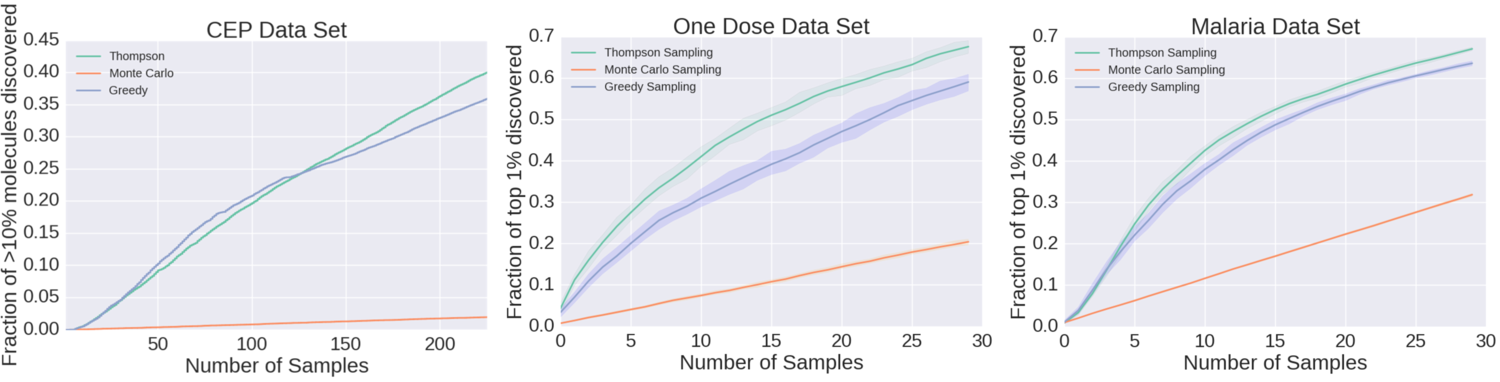
\includegraphics[width=0.8\columnwidth]{figures/thompson_tile/thompson_tile3.png}
\label{fig:thompson_1pc}
\caption{The recall of the Thompson sampling methodology for each of the datasets included in this study.  For the CEP dataset, the recall for molecules with a PCE $>10\%$ is reported, whilst for the One-Dose and Malaria datasets the recall for the top 1\% of targets is reported.  In addition to the baseline Monte Carlo sampling, we also include a greedy sampling approach, in which there is no exploration, but the training set is selected by exploiting the predictive power of the model.  The general lower performance of this model indicates the importance of balancing exploration and exploitation when choosing molecules for high-throughput virtual screening.}
\end{center}
\end{figure}
This effect can be seen more clearly in Figure \ref{fig:cep_lib}.  The greedy strategy (green) initially performs exceptionally well, with a significant enrichment over both Monte Carlo and Thompson sampling strategies.  This advantage quickly decays, however, as the Thompson sampling benefits from the exploration performed, and the derived improved description of potential desirable areas of chemical space. We emphasize that even the Clean Energy Project, with its strongly localized cluster of desirable molecules, demonstrates deficiencies in the greedy sampling strategy.  Indeed, some of the strength shown by the greedy sampling strategy can be attributed to the sheer size of the dataset, with respect to the others investigated within this study.  It is logical that a method whose strength lies in exploiting localized knowledge of an area of chemical space in which desirable molecules have been found will benefit from a dataset which contains a large number of molecules, and which has been designed combinatorially. It should also be noted that the success of a greedy methodology is also dependent on the existence of a wide-necked funnel in the information landscape - if a cluster of desirable molecules in chemical space is too tight, it is unlikely to be sampled in the initialization of the method.  Thus, it is unlikely to be discovered - at least in an `intelligent' manner - by a greedy sampling methodology; a situation which is strongly undesirable when building libraries for which each point is expensive to discover the ground truth value.
  

\begin{figure}[htb]
\begin{center}
\includegraphics[width=0.9\columnwidth]{figures/thompson_cep_lib/thompson_cep_lib2.png}
\label{fig:cep_lib}
\caption{The fraction of the library - built with either the greedy methodology, Thompson sampling, or Monte Carlo - which contains extreme molecules (here, defined as $> 10\%$ power conversion efficiency).  Whilst the greedy methodology is initially very successful, its performance drops sharply after the initially discovered desirable area of chemical space is exhausted of molecules.}
\end{center}
\end{figure}

In order to put the importance of these results into context, we consider the saving in calculation time for the Clean Energy Project dataset. Thompson sampling, displays $>30x$ faster discovery than the Monte Carlo search, which is in itself faster than the exhaustive enumeration used in the initial exploration of this dataset. Even assuming a discovery rate of 30 times as fast as the initial Clean Energy Project, which we belive to be conservative, 34,000 CPU years would have been saved in exploring this part of chemical space.  

Both the One-Dose and Malaria datasets contain around 20,000 molecules; yet by using Thompson sampling, we can locate 70\% of the highly active molecules in both sets, by sampling only 600 molecules. This represents a huge reduction in the discovery time for new theraputic molecules, not to mention a significant saving in the economic costs associated with synthesiszing and testing these molecules.

\section{Conclusion}
We describe a method which utilizes techniques derived from information theory and machine learning to guide an intelligent search of local areas of chemical space, and its application to the discovery of novel photovoltaic materials and therapeutic molecules.  In order to understand the performance of these intelligent searching methods, we also present a novel component reduction algorithm, based upon the use of unsupervised neural networks.  This demonstrates the diversity of the datasets through the eyes of a neural network, and provides a means of analysing diversity through the components which are most strongly expressed through the neural network.  

Our results demonstrate how the underlying uncertainty in predictive values can be exploited through the use of maximum entropy sampling to provide the which optimially balance predictive power against the size of the molecular library. If the search can be formulated as a classic optimization problem, we show how Thompson sampling can be used to quickly and robustly locate extreme molecules by balancing exploration of the underlying information, with exploitation of the predictive model provided by a Bayesian neural network. This resulted in significant increases in the rate of discovery, displaying significant potential for improving the current model of molecular discovery, especially within the virtual realm.


\bibliography{bibliography/converted_to_latex2}

\end{document}

